%%----------------------------------------------------------------------------
%% Presentatie HoGent Bedrijf en Organisatie
%%----------------------------------------------------------------------------
%% Auteur: Bert Van Vreckem [bert.vanvreckem@hogent.be]

\documentclass{beamer}

%==============================================================================
% Aanloop
%==============================================================================

%---------- Packages ----------------------------------------------------------
\usepackage{etex}
\usepackage{graphicx,multicol}
\usepackage{comment,enumerate,hyperref}
\usepackage{amsmath,amsfonts,amssymb}
\usepackage{tikz}
\usepackage[english]{babel}
\usepackage[utf8]{inputenc}
\usepackage{multirow}
\usepackage{eurosym}
\usepackage{listings}
\usepackage[T1]{fontenc}
\usepackage{lmodern}
\usepackage{textcomp}
\usepackage{framed}
\usepackage{wrapfig}
\usepackage{pgf-pie}
\usepackage{pgfplots}
\usepackage{booktabs}
\usepackage{pgfplotstable}
\usepackage{changepage}
\usepackage{pst-plot,pst-func}

%---------- Configuratie ------------------------------------------------------

\usetikzlibrary{arrows,shapes,backgrounds,positioning,shadows}
\usetikzlibrary{pgfplots.statistics}
\newif\ifprivate
\privatetrue


\usetheme{hogent}
\setbeameroption{show notes}

%---------- Commando-definities -----------------------------------------------

\newcommand{\tabitem}{~~\llap{\textbullet}~~}
\renewcommand{\arraystretch}{1.2}

%---------- Info over de presentatie ------------------------------------------

\title[Intro]{Research techniques\\Time series}
\author{Anita Bernard, Jens Buysse, Bert {Van Vreckem}}
\date{AY 2016-2017}

%==============================================================================
% Inhoud presentatie
%==============================================================================

\begin{document}

%---------- Front matter ------------------------------------------------------

% Dia met het HoGent logo
\HoGentLogo

% Titeldia met faculteitslogo
\titleframe

%---------- Inhoud ------------------------------------------------------------

\begin{frame}
  \frametitle{What's on the menu today?}

  \tableofcontents
\end{frame}

\section{Time series and predictions}

\begin{frame}
  \frametitle{Time series and predictions}

  \brightbox{A time series is a sequence of observations of a variable over time}

  A time series is a stochastic process. Examples include:

  \begin{itemize}
    \item Monthly demand for milk
    \item Yearly influx of ``generational students'' in a college
    \item The price of a stock or bond at the stock exchange (day to day, hour to hour, etc.)
    \item The number of HTTP requests per second on a website, or the response time for those requests
    \item Evolution of disk usage on a backup server
  \end{itemize}
\end{frame}

\begin{frame}
  \frametitle{Time series and predictions}
  
  Time series are an important part of research, because the often are the \emph{foundation} of decision models and predictions.
  
  \begin{itemize}
    \item Capacity planning (e.g. disk storage, computing power)
    \item Reaching financial objectives, a.o.~investments
    \item Planning operational/marketing budgets
    \item \dots
  \end{itemize}
\end{frame}

\begin{frame}
  \frametitle{Time series and predictions}

  Time series are a \emph{statistical} problem: observations will vary over time.
  
  \begin{figure}
    \centering
    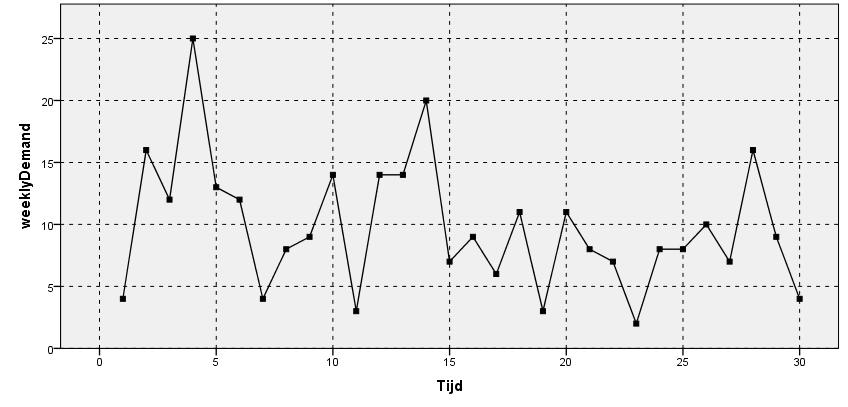
\includegraphics[width=\textwidth]{img/tijdreeks11}
    \caption{Time series for the weekly demand for some product.}
  \end{figure}
\end{frame}

\section{Time series models}

\subsection{Mathematical model}

\begin{frame}
  \frametitle{Mathematical models for time series}

  The simplest model:

  \begin{itemize}
    \item Constant $b$
    \item Variations around $b$, modeled by a random variable $\varepsilon_{t}$
  \end{itemize}

  \begin{equation}
    X_{t} = b + \varepsilon_{t}
    \label{eq:timeseries-constant}
  \end{equation}

  \begin{itemize}
    \item $X_{t}$: stochastic variable for the time series, at time $t$
    \item $x_{t}$: \emph{observation} at time $t$
    \item $\varepsilon_{t}$: \emph{noise}. We assume $\varepsilon_{t} \sim Nor(\mu = 0; \sigma)$
  \end{itemize}
\end{frame}

\begin{frame}
  \frametitle{Mathematical models for time series}

  We can also assume a linear relation:
  
  \begin{equation}
    X_{t} = b_{0} + b_{1} \times t + \varepsilon_{t}
    \label{eq:timeseries-linear}
  \end{equation}

  Equations~\ref{eq:timeseries-constant} and \ref{eq:timeseries-linear} are specific instances of the more general \emph{polynomial} case:

  \begin{equation}
    X_{t} = b_{0} + b_{1} t + b_{2} t^{2} + \dots + b_{n} t^{n} + \varepsilon_{t}
    \label{eq:timeseries-polynomial}
  \end{equation}
\end{frame}

\subsection{General}

\begin{frame}
  \frametitle{General parametric model for time series}

  A time series is a function with parameters $b_i$.

  \begin{equation}
    X_{t} = f(b_{0}, b_{1}, b_{2}, \dots , b_{n}, t) + \varepsilon_{t}
    \label{eq:timeseries-parametric}
  \end{equation}

  We also assume:

  \begin{itemize}
    \item We consider two components of variability:
      \begin{itemize}
        \item the average of the variable varies over time
        \item there is random variation w.r.t.~this mean
      \end{itemize}
    \item The variance of the residuals in the model ($X_t - x_t$) is constant over time (\emph{homeoscedastic})
  \end{itemize}
\end{frame}

\subsection{Parameter estimation}

\begin{frame}
  \frametitle{Parameter estimation}

  Goal = to make predictions based on the time series model (forecasting)

  \begin{enumerate}
    \item select the most appropriate parametric model
    \item estimate the parameters $b_i (i: 1, \dots, n)$ based on the
  \end{enumerate}

  These estimates $\widehat{b_i}$ are chosen in a way that they approach the observations as well as possible.
\end{frame}

\begin{frame}
  \frametitle{Parameter estimation: example}

  \begin{table}[t]
    \centering
    \begin{tabular}{|l|l|l|l|l|l|l|l|l|l|}
      \hline
      4 & 16 & 12 & 25 & 13 & 12 & 4 & 8  & 9 & 14 \\ \hline
      3 & 14 & 14 & 20 & 7  & 9  & 6 & 11 & 3 & 11 \\ \hline
      8 & 7  & 2  & 8  & 8  & 10 & 7 & 16 & 9 & 4  \\ \hline
    \end{tabular}
    \label{tab:data}
    \caption{Time series of the weekly demand for some product}
  \end{table}

  \begin{figure}
    \centering
    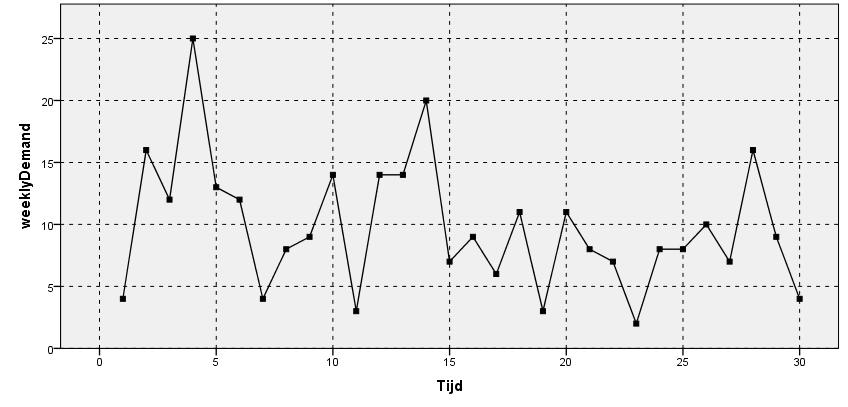
\includegraphics[width=.7\textwidth]{img/tijdreeks11}
  \end{figure}
\end{frame}

\begin{frame}
  \frametitle{Parameter estimation: example}

  \begin{itemize}
    \item We choose the constant model from Equation~\ref{eq:timeseries-constant}
    \item As estimate for $b$, we choose the average of the first 20 observations:

      \[ \widehat{b} = \frac{1}{20} \sum_{t = 1}^{20} x_{t}= 10.75 \]

  \end{itemize}

  \centering
  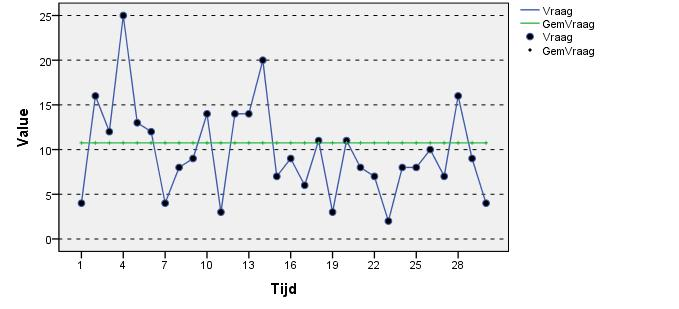
\includegraphics[width=.7\textwidth]{img/tijdreeks21.jpg}
\end{frame}

\begin{frame}
  \frametitle{Parameter estimation: example}

  The observations used for the estimate of $\widehat{b}$ can be chosen, e.g.:

  \begin{itemize}
    \item $\widehat{b} = \frac{1}{10} \sum_{10}^{20} x_{t} = 10.18$
    \item $\widehat{b} = \frac{1}{5} \sum_{15}^{20} x_{t} = 7.83$
  \end{itemize}

\end{frame}

\section{Moving average}

\subsection{Simple moving average (SMA)}

\begin{frame}
  \frametitle{Simple Moving average}

  \brightbox{The \textcolor{HoGentYellow}{Simple Moving Average} is a series of \emph{averages} of the last $m$ observations}

  \begin{itemize}
    \item Hide short term fluctuations and show long term trends
    \item $m$ is the time range, and is the parameter of this method
  \end{itemize}

  \begin{equation}
    SMA(t) = \sum_{i=k}^{t} \frac{x_{i}}{m}
    \label{eq:movingAverage}
  \end{equation}

  met $k = t - m + 1$.
\end{frame}

\begin{frame}
  \frametitle{Application: ``Golden cross''}

  Moving Averages are used in the \emph{technical analysis} of stock prices in order to discover trends.

  \begin{center}
    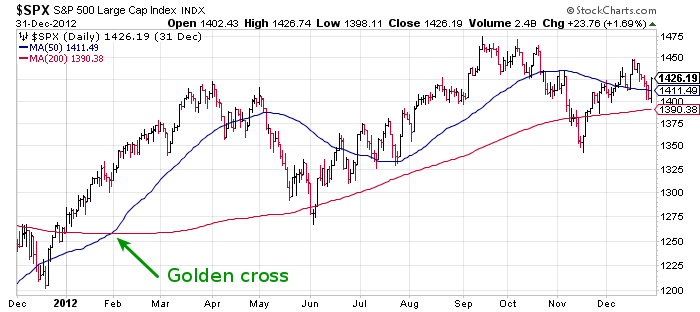
\includegraphics[width=\textwidth]{img/tijdreeks-golden-cross}
  \end{center}
\end{frame}

\note{%
  This chart shows the evolution of the S\&P500 index (compare to Bel-20, Euro Stoxx 50) from December 2011 to the end of 2012. The chart shows the SMA's of the price at closing time of the 50 and 200 last trade days (notated: MA(50) and MA(200)). When the market is in a downward trend (``\textbf{bear market}''), the MA(200) is above MA(50) (see left part of the chart).

  In February 2012, the MA(50) rose above the MA(200), an event that is called a ``\textbf{golden cross}''. The increase of the index had started a few months earlier, but the MA's obviously are slower.
  
  A \emph{golden cross} is an indicator that the market (or a specific traded equity) is in a long term upward trend (``\textbf{bull market}''). In this case, the trend lasts up to the present day (spring of 2017).

  The MA(200)-line is considerd to be a support, i.e.~a lower bound for the stock price. At this level, the stock price is appealing, so demand typically rises and the price is pulled up again. That is, if the circumstances haven't changed (the stock's \emph{fundamentals}, economy in general, \dots).

}

\begin{frame}
  \begin{table}
    \begin{tabular}{|llllllllll|}
      \hline
      ~       & 11   & 12   & 13   & 14   & 15   & 16   & 17   & 18   & 19   \\
      $x_{t}$ & 3    & 14   & 14   & 20   & 7    & 9    & 6    & 11   & 3    \\
      $X_{t}$ & 11.7 & 11.6 & 11.4 & 11.6 & 11.1 & 10.5 & 10.2 & 10.4 & 10.7 \\
      $e$     & -8.7 & 2.4  & 2.6  & 8.4  & -4.1 & -1.5 & -4.2 & 0.6  & -7.7 \\ \hline
    \end{tabular}
    \caption{Error in moving average ($m = 10$) predictions.}
    \label{tab:error}
\end{table}

A method to measure the quality of the predictions is the mean absolute devations (MAD):

\begin{equation}
  MAD = \frac{1}{n} \sum_{1}^{n} \left| e_{i} \right|
\label{eq:MAD}
\end{equation}

You can also calculate the mean squared deviation/mean squared error (MSE):

\begin{equation}
  s^{2}_{e} = \frac{1}{m} \sum_{1}^{n} (e_{i} - \overline{e})^{2}
\label{eq:varError}
\end{equation}
\end{frame}

\subsection{Weighted Moving Average}

\begin{frame}
  \frametitle{Weighted Moving Average}

  \begin{itemize}
    \item In the case of $SMA$ all observations contribute equally
    \item Weighted Moving Average ($WMA$) has multiplying factors to give different weights to observations
    \item A special case is the \emph{Exponential Moving Average} ($EMA$) or \emph{exponential smoothing}:
      \begin{equation}
        EMA(t) = \alpha x_{t-1} + (1-\alpha) EMA(t-1)
        \label{eq:singleExpMA}
      \end{equation}

      with $\alpha$ the smoothing constant ($0 < \alpha < 1$), and $t \geq 3$
  \end{itemize}
\end{frame}

\begin{frame}
  \frametitle{Exponential Moving Average}

  Formula~\ref{eq:singleExpMA} is only valid from $t=3$. Determining  $EMA(2)$ is an important parameter. Some possible choices:
  
  \begin{itemize}
    \item $EMA(2) = x_1$
    \item $EMA(2) = \frac{1}{m} \sum_{i=1}^{m} x_i$ (i.e.~mean of the first $m$ observations)
    \item Set $EMA(2)$ to some objective value
    \item \ldots
  \end{itemize}
\end{frame}

\begin{frame}
  \frametitle{Why ``\emph{exponential}''?}

  \begin{align*}
    EMA(t) & = \alpha x_{t-1} + (1-\alpha) EMA(t-1)                                           \\ \pause
           & = \alpha x_{t-1} + (1-\alpha)\left[\alpha x_{t-2} + (1-\alpha)EMA(t - 2)\right]  \\ \pause
           & = \alpha x_{t-1} + \alpha (1-\alpha)x_{t-2} + (1-\alpha)^{2} EMA(t - 2)          \\ \pause
           &   \text{or, in general:} \\ \pause
           & = \alpha \sum_{i=1}^{t-2}(1-\alpha)^{i-1}x_{t-i} + (1-\alpha)^{t-2} EMA(2), t \geq 2
  \end{align*}

  The weight of older observations decreases exponentially
\end{frame}

\begin{frame}
  \frametitle{Exponential smoothing}

  \begin{table}
    \centering
    \begin{tabular}{l|llll}
      $\alpha$ & $(1-\alpha)$ & $(1-\alpha)^{2}$ & $(1-\alpha)^{3}$ & $(1-\alpha)^{4}$ \\ \hline
      0.9   & 0.1       & 0.01             & 0.001                      & 0.0001           \\
      0.5   & 0.5       & 0.25             & 0.125                      & 0.062            \\
      0.1   & 0.9       & 0.81             & 0.729                      & 0.6561           \\
    \end{tabular}
    \caption{Values for $\alpha$ and $(1-\alpha)^{n}$}
    \label{tab:alpha}
  \end{table}
  How quickly old observations are ``forgotten'' depends on $\alpha$. With $\alpha$ close to 1, old values are forgotten quickly, with $\alpha$ close to 0, older values are ``remembered'' longer.
\end{frame}


\begin{frame}
  \frametitle{Example}
  \begin{figure}[htbp]
    \centering
    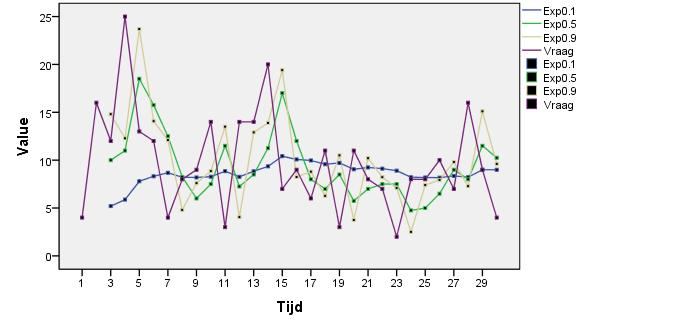
\includegraphics[width=\textwidth]{img/tijdreeks51}
    \caption{Exponential moving averages with $\alpha=0.1 , 0.5, 0.9$}
    \label{fig:tijdreeks51}
  \end{figure}
\end{frame}

\subsection{Double exponential smoothing}

\begin{frame}
  \frametitle{Double exponential smoothing}

  When there's a trend in the data, exponential smoothing doesn't work very well
  
  \begin{figure}
    \centering
    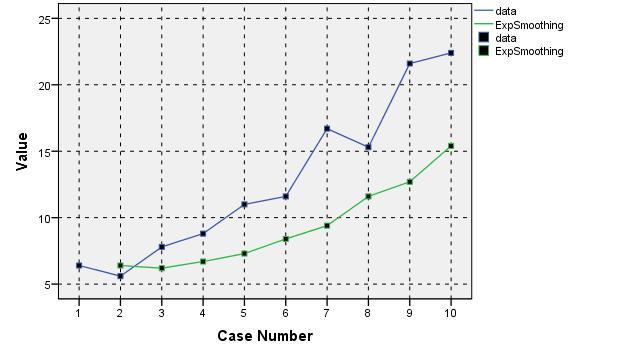
\includegraphics[width=.7\textwidth]{img/tijdreeks61}
    \caption{Exponential smoothing with a trend: errors increase}
    \label{fig:tijdreeks61}
  \end{figure}

\end{frame}


\begin{frame}
  \frametitle{Double exponential smoothing}
  
  We introduce an extra term in the model to estimate the trend: $b_t$ at time $t > 1$:

\begin{eqnarray}
  X_{t} = \alpha x_{t} + (1-\alpha)(X_{t-1} + b_{t-1}) & 0 \leq \alpha \leq 1 \\
  b_{t} = \gamma(X_{t}-X_{t-1}) + (1-\gamma)b_{t-1} & 0 \leq \gamma \leq 1 
\label{eq:doubleSmoothing}
\end{eqnarray}

  with $0 < \alpha < 1$ and $0 < \gamma < 1$
  
  \begin{itemize}
    \item $ b_{t-1}$ in the first equation ensures estimates follow the trend
    \item $X_{t}-X_{t-1}$ is positive or negative and is used to update the trend estimate
  \end{itemize}
\end{frame}

\begin{frame}
  \frametitle{Double exponential smoothing}
  
  Alternatives for bootstrapping:
  
\begin{align*}
  X_{1} & = x_{1} \\
  b_{1} & = x_{2} - x_{1} \\
  b_{1} & = \frac{1}{3}\left[ (x_{2} - x_{1}) + (x_{1} - x_{2}) + (x_{4} - x_{3}) \right]\\
  b_{1} & = \frac{x_{n} - x_{1}}{n-1} \\
\end{align*}

\end{frame}

\subsubsection{Forecasting}

\begin{frame}
  \frametitle{Forecasting}
  
  To determine a forecast $F(t+1)$ for time index $t+1$, we use:

  \[ F(t+1) = s_t + b_t \]

  or in general, for time index $t+m$:

  \[ F(t+m) = s_t + m b_t \]
\end{frame}

\begin{frame}
  \begin{figure}
    \centering
    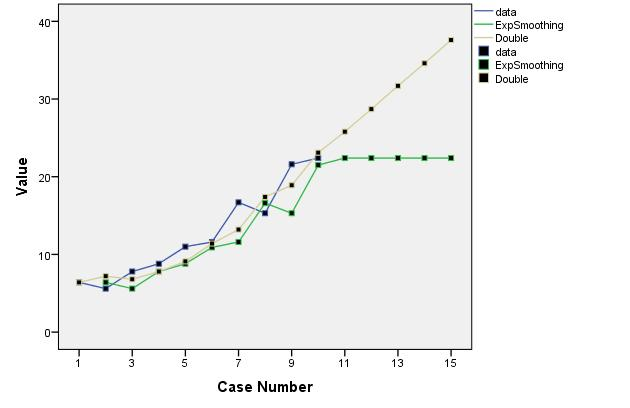
\includegraphics[width=\textwidth]{img/tijdreeks71}
    \caption{Basic and double exponential smoothing}
    \label{fig:tijdreeks71}
  \end{figure}
\end{frame}

\subsection{Triple exponential smoothing}

\begin{frame}
  \frametitle{Triple exponential smoothing}
  also called Holt-Winters filtering. Also takes seasonality into account.

  \begin{itemize}
    \item $L$: length of the seasonal cycle (number of time units)
    \item $c_t$: term modeling the seasonal variations
    \item $\gamma$: smoothing factor for the seasonal variation
  \end{itemize}

\begin{align*}
  X_{t} &= \alpha \frac{x_{t}}{c_{t-L}} + (1-\alpha) (X_{t-1} + b_{t-1}) & \textnormal{Smoothing}\\
  b_{t} &= \gamma (X_{t} - X_{t-1}) + (1-\gamma)b_{t-1} & \textnormal{Trend smoothing} \\
  c_{t} &= \beta \frac{x_{t}}{X_{t}} + (1-\beta)c_{t-L} & \textnormal{Seasonal smoothing} \\
\label{eq:HoltWinters}
\end{align*}

\end{frame}

\begin{frame}
  \frametitle{Triple exponential smoothing}

  Forecast at time $t + m$:

  \[ F_{t+m} = (X_{t} + mb_{t})c_{t-L+m} \]

  For an implementation in Java, see \url{https://github.com/bertvv/wintersmethod}
\end{frame}

\begin{frame}
  \frametitle{Example: sales forecast}

  \centering
  \begin{tikzpicture}
    \begin{axis}[
        title=Observed sales figures,
        xlabel=Weekday,
        ylabel=SKUs,
      ]
      \addplot table [x index=0, y index=1, col sep=comma] {data/shoestore-sales.dat};
    \end{axis}
  \end{tikzpicture}
\end{frame}

\begin{frame}
  \frametitle{Example: sales forecast}

  Keuze startwaarden:

  \begin{itemize}
    \item smoothing factors: $\alpha = 0.8, \beta = 0.8, \gamma = 0.3$
    \item $s_0 = 5849$, $b_0 = 123.3$
    \item $L = 7$ (i.e.~weekly repetition), so we need 7 values to initialise $c_t$ (see Table~\ref{tab:winters-init-c})
  \end{itemize}

  \begin{table}
    \centering
    \begin{tabular}{l|l|l|l}
      Mon ($c_0$) & Tue ($c_1$) & Wed ($c_2$) & Thu ($c_3$)  \\
      1.245693 & 1.115265 & 1.088853 & 1.135378 \\
      \hline \hline
      Fri ($c_4$)  & Sat ($c_5$)  & Sun ($c_6$)  & \\
      1.178552 & 1.229739 & 0.006520 &
    \end{tabular}
    \caption{Initial values for $c_t$}
    \label{tab:winters-init-c}
  \end{table}
\end{frame}

\begin{frame}
  \frametitle{Example: sales forecast}


  \begin{center}
  \begin{tikzpicture}
    \begin{axis}[
        scale=.8,
        title=Sales figures,
        xlabel=Weekday,
        ylabel=SKUs,
        unbounded coords=jump,
        legend to name=bottomlegend,
      ]
      \addplot table [x index=0, y index=1, col sep=comma] {data/shoestore-sales.dat};
      \addlegendentry{Observed}
      \addplot table [x index=0, y index=2, col sep=comma] {data/shoestore-sales.dat};
      \addlegendentry{Predicted}
    \end{axis}
  \end{tikzpicture}

  \ref{bottomlegend}
\end{center}

\end{frame}


\end{document}

